%!TEX root = MagicSquare.tex
We assume a basic familiarity with quantum information, see e.g.\ \cite{nielsen2002quantum}. We introduce all necessary notions from the fields of nonlocal games and self-testing, but we don't reproduce all of the proofs.


% With respect to this definition, we obtain the first known nonlocal game capable of self-testing maximally entangled qudits of dimension $d$ for arbitrary $d$.
% For generalized correlations, letting $V$ output values in the interval $[0,1]$, Coladangelo, Goh, and Scarani \cite{coladangelo2016all} already achieve this. Furthermore, their test only requires one pair of qudits.
\subsection{Notation}
We write $[n]$ to refer to the finite set $\set{1,\ldots, n}$ with $n$ elements. We write $[A,B]$ for $ABA\1B\1$, the group commutator of $A$ and $B$.
We use the Dirac delta notation 
\begin{equation}
	\delta_{x,y} :=\begin{cases}
		1, &\text{ if }x=y\\
		0, &\text{ otherwise}
	\end{cases}.
\end{equation}
$\mathbf H$ will refer to a hypergraph, while 
$\m H$ will refer to a Hilbert space.
$\m L(\m H)$ is the space of linear operators on the Hilbert space $\m H$. 
%$e$ will refer to an edge of a hypergraph or variable of a linear constraint game. $v$ will refer to a vertex of a hypergraph or a constraint of an LCS game. $1$ will refer to the identity element of a group. 
$\rho$ will always refer to a state on a Hilbert space, while $\s$ and $\tau$ are reserved for group representations. $\w_d:= e^{2\pi i /d}$ will always refer to the same $d\th$ root of unity. 
When we have multiple Hilbert spaces, we label them with subscripts, e.g.\ as $\m H_A, \m H_B$. In that case, we may also put subscripts on operators and states to indicate which Hilbert spaces they are associated with. 
When the Hilbert space is clear from context, $I$ refers to the identity operator on that space. 
$I_d$ will always refer to the identity operator on $\C^d$. 
$\eprp:=\frac{1}{\sqrt d}\sum_i^d\ket{ii}$ refers to the maximally entangled state on $\C^d\otimes \C^d$. We use the shorthand $\Tr_\rho(X) = \Tr X\rho$. 
We use the following notion of state-dependent distance, which we'll recall, and prove properties of, in \S\ref{subsection:state-dependent-distance}.
\begin{equation}\label{eq:state-dependent-distance-definition}
	\drho{\rho}{X}{Y} = \sqrt{\Tr_\rho(X-Y)^\dagger(X-Y)}.
\end{equation}
$\norm{X}_p$ denotes the $p$-norm of $X$, i.e.\ $\norm X_1 = \Tr\sqrt{XX^\dagger}$ and $\norm X_2 = \sqrt{\Tr XX^\dagger}$.

\subsection{Nonlocal games}

\begin{definition}[Nonlocal game]
	For our purposes, a nonlocal game $G$ is a tuple $(A,B,X,Y,V,\pi)$, where $A,B,X,Y$ are finite sets of answers and questions for Alice and Bob, $\pi:X\times Y\to [0,1]$ is a probability distribution over questions, and $V:A\times B \times X \times Y\to \pair01$ is \emph{the win condition}. 
\end{definition}

\begin{definition}[Strategies for nonlocal games]
	If $G$ is a nonlocal game, then a strategy for $G$ is a probability distribution $p:A\times B\times X\times Y\to [0,1]$.	The \emph{value} or \emph{winning probability} of a strategy is given by 
	\begin{equation}
		\w(G;p) := \sum_{a,b,x,y}\pi(x,y)p(a,b\|x,y)V(a,b,x,y).
	\end{equation}
	If the value is equal to $1$, we say that the strategy is \emph{perfect}. If the probability distribution is separable, i.e.\ $p(a,b\|x,y) = \sum \a_i p_i(a\|x)q_i(b\|y)$ for some probability distributions $\set{p_i}, \set{q_i}$, then we say that the strategy is \emph{local}.
\end{definition}
	%Operationally, we think of the value of a strategy as the probability that provers using the strategy win the game. 
	We think of a local strategy as being implemented by using only the resource of public shared randomness. Alternatively, the local strategies are the strategies which are implementable by spacelike-separated parties in a hidden variable theory of physics.
\begin{definition}[Quantum strategies, projective measurement version]
	We say that a strategy $p:A\times B\times X\times Y\to [0,1]$ is \emph{quantum of local dimension $d$} if there exist projective measurements $\set{\set{A_x^a}_a}_x, \set{\set{B_y^b}_b}_y$ on $\C^d$ and a state $\rho \in \m L(\C^d\otimes \C^d)$ such that 
	\begin{equation}
		p(a,b\|x,y) = \Tr_\rho(A_x^a\otimes B_y^b)
	\end{equation}
	 (By \emph{projective measurement} we mean that for all $x,y,a,b$ we have $(A_x^a)^2 = A_x^a = (A_x^a)\dagg, (B_y^b)^2 = B^b_y= (B^b_y)\dagg$, and for all $x,y$, we have $\sum_a A_x^a = I = \sum_bB_y^b$.)
	 \\\noindent We say that a strategy is \emph{quantum} if it is quantum of local dimension $d$ for some $d$.
\end{definition}
We denote by $\w_*(G)$ the \emph{optimal quantum value} of $G$, i.e. the supremum over all quantum strategies of the winning probability. If the value of a strategy is $\w_*(G)$, we say that the strategy is \emph{ideal}. For quantum strategies, we use the term \emph{strategy} to refer interchangeably to the probability distribution or to the state and measurement operators producing it. 

% We'll sometimes find it useful to present quantum strategies by a set of unitary observables instead of by a set of projective measurements.
% \begin{definition}[Quantum strategy, observable version]
% 	$\set{\set{A_x^a}_a}_x, \set{\set{B_y^b}_b}_y$ on $\C^d$ and a state $\rho \in \m L(\C^d\otimes \C^d)$
	
% \end{definition}

% \begin{prop}
% 	The projective measurement and unitary observable strategies are equivalent. More precisely, there is a one-to-one correspondence between projective measurement strategies and unitary observable strategies producing the same correlation.
% \end{prop}
% \begin{proof}
	
% \end{proof}


\begin{definition}[Self-testing]
We say that a non-local game $G$ \emph{self-tests} a quantum strategy $S = (\set{\set{A_x^a}_a}_x, \set{\set{B_y^b}_b}_y, \ket{\Psi}) $ if any quantum strategy $S'$ that achieves the optimal quantum winning probability $w_*$ is equivalent up to local isometry to $S$.
\end{definition}
By \emph{local isometry} we mean a channel $\Phi: \m L(\m H_A\otimes \m H_B) \to \m L(\m H_A'\otimes \m H_B')$ which factors as $\Phi(\rho) = (V_A\otimes V_B) \rho(V_A\otimes V_B)^\dagger$, where $V_A: \m H_A\to \m H_A', V_B: \m H_B\to \m H_B'$ are isometries.

\begin{definition}[Robustness of self-tests] We say that a non-local game $G$ is $\left(\eps,\delta(\eps)\right)$-rigid if it self-tests a strategy $S = (\set{\set{A_x^a}_a}_x, \set{\set{B_y^b}_b}_y, \ket{\Psi})$, and, moreover, for any quantum strategy $\tilde{S} = \big(\set{\set{\tilde{A}_x^{a}}_a}_x, \set{\set{\tilde{B}_y^{b}}_b}_y, \rho \big)$ that achieves a winning probability of $w_*(G) - \eps$, there exists a local isometry $\Phi$ such that 
\begin{equation}
\norm {\Phi(\tilde{A}_x^{a}\otimes \tilde{B}_y^{b}\ \rho \tilde{A}_x^{a}\otimes \tilde{B}_y^{b}) - \big(A_x^a\otimes B_y^b \ket{\Psi}\bra{\Psi} A_x^a\otimes B_y^b \big)\otimes \rho_{\text{extra}}}_{2} \leq \delta(\eps)
\end{equation}
where $\rho_{\text{extra}}$ is some auxiliary state, and $\delta(\eps)$ is a function that goes to zero with $\eps$.
\end{definition}
\subsection{Groups}

We work with several groups via their presentations. For the basic definitions of group, quotient group, etc.\ see any abstract algebra text, e.g.\ \cite{dummit2004abstract}.
\begin{definition}
	Let $S$ be a set of letters. We denote by $\m F(S)$ the \emph{free group on $S$}. As a set, $\m F(S)$ consists of all finite words made from $\set{s,s\1\;s\in S}$ such that no $ss\1$ or $s\1s$ appears as a substring for any $s$. The group law is given by concatenation and cancellation.
\end{definition}


\begin{definition}[Group presentation]
	Let $S$ be finite and $R$ a finite subset of $\m F(S)$. Then $G = \Braket {S:R}$ is the \emph{finitely presented group} generated by $S$ with relations from $R$. Explicitly, 
	$G = \m F(S)/\braket R$, where $/$ is used to denote the quotient of groups, and $\braket R$ denotes the subgroup generated by $R$. 
	We say that an equation $w = w'$ is \emph{witnessed by $R$} if $w'w^{-1}$ (or some cyclic permutation thereof) is a member of $R$. 
\end{definition}
We emphasize that in this work, we sometimes distinguish between two presentations of the same group. If $G = \braket{S:R}, G' = \braket{S':R'}$ are two finitely presented groups, we reserve equality for the case $S = S'$ and $R = R'$, and in this case we'll say $G = G'$. We'll say that $G \cong G'$ if there is a group isomorphism between them.


\begin{definition}\label{definition:canonical-form}
	Let $G = \braket{S:R}$ be a finitely presented group and $\can: G\to \m F(S)$ be an injective function. We say that $\can$ is a \emph{canonical form} for $G$ if the induced map $\bar \can: G\to \m F(S)/\braket{R}$ is an isomorphism. In other words, we require that $\can(g)\can(h) = \can(gh)$ as elements of $G$, but not as strings.
\end{definition}

Now and throughout the paper, for a group $G$, we'll denote by $1$ its identity, and we'll let $[a,b] := aba\1b\1$ denote the commutator of $a$ and $b$. The group presentations of interest in this paper will take a special form extending the ``groups presented over $\Z_2$'' from \cite{slofstra2016tsirelson}. %The following definitions are valid for any integer $p$, but in the remainder of the paper, we'll only be interested in the case that $p$ is prime.

\begin{definition}[Group presentation over $\Z_d$]
	Let $d\in \N$ and let $\Z_d = \Braket{J:J^d}$ be the finite cyclic group of order $d$. A \emph{group presented over $\Z_d$} is a group $G = \Braket{S':R'}$, where $S'$ contains a distinguished element $J$ and $R'$ contains relations $[s,J]$ and $s^d$ for all $s\in S$.
	
	For convenience, we introduce notation that suppresses the standard generator $J$ and the standard relations.
	\begin{equation}
		G= \Braket{S:R}_{\Z_d} = \Braket{
		S\cup\set{ J } : R \cup \set{ s^d,J^d,[s,J] \; s\in S }
		}
	\end{equation}
\end{definition}
In the group representations of interest, we'll have $J \mapsto e^{2\pi i/d}$---we should always just think of $J$ as a $d\th$ root of unity. We'll think of relations of the form $J\1[a,b]$ as ``twisted commutation'' relations, since they enforce the equation $aba\1b\1 = e^{2\pi i/d}$.

\begin{example}\label{example:P_d}
	The Pauli group on one $d$-dimensional qudit can be presented as a group over $\Z_{d}$. 
	\begin{equation}
	\m P_d^{\otimes 1} = \Braket{x,z: J[x,z]}_{\Z_{d}}
	\end{equation}
\end{example}

\subsection{Group pictures}\label{subsection:van-kampen-diagrams}

Suppose we have a finitely presented group $G = \braket{S:R}$ and a word $w\in \m F(S)$ such that $w = 1$ in $G$. 
Then by definition, there is a way to prove that $w = 1$ using the relations from $R$. How complicated can such a proof get? Group pictures give us a way to deal with these proofs graphically, rather than by writing long strings of equations.
In particular, we will use group pictures to get quantitative bounds on the length of such proofs. (For a more mathematically rigorous treatment of group pictures, see \cite{slofstra2016tsirelson}. These are dual to what are usually known as van Kampen diagrams.) 

\begin{definition}[Group picture]
	Let $G = \Braket{S:R}_{\Z_d}$ be a group presented over $\Z_d$. A $G$-picture is a labeled drawing of a planar directed graph in the disk. Some vertices may lie on the boundary. The vertices that do not lie on the boundary are referred to as \emph{interior vertices}. A $G$-picture is \emph{valid} if the following conditions hold:
	\begin{itemize}
		\item Each interior vertex is labeled with a power of $J$. (We omit the identity label.)
		\item Each edge is labeled with a generator from $S$.
		\item At each interior vertex $v$, 
		% the following procedure forms a relation $r\in R$.
		the clockwise product of the edge labels (an edge labeled $s$ should be interpreted as $s$ if it is outgoing and as $s\1$ if it is ingoing) is equal to the vertex label, as witnessed by $R$. (Since the values of the labels are in the center of the group, it doesn't matter where you choose to start the word.)
	\end{itemize}
\end{definition}
% A group picture is not a picture containing all of the information 
Note that the validity of a $G$-picture depends on the presentation of $G$. Pictures cannot be associated directly with abstract groups.

If we collapse the boundary of the disk to a point (``the point at infinity''), then the picture becomes an embedding of a planar graph on the sphere (see Figure \ref{fig:sphere}). The following is a kind of ``Stoke's theorem'' for group pictures, which tells us that the relation encoded at the point at infinity is always valid.

\begin{figure}
	\begin{center}
	\begin{tabular}{m{0.5\textwidth}m{0.5\textwidth}}
	    \resizebox{0.5\textwidth}{!}{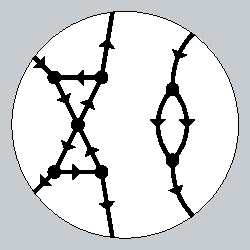
\includegraphics{MagicSquare-figure3.pdf}}
	    &
	    \resizebox{0.5\textwidth}{!}{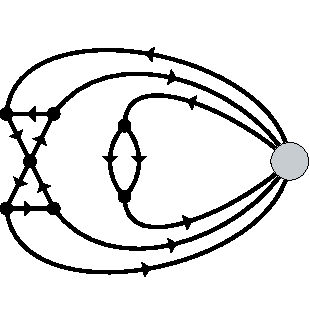
\includegraphics{MagicSquare-figure4.pdf}}
	\end{tabular}
    \end{center}
    \caption{This is a directed version of Figure 3 from \cite{slofstra2016tsirelson}
    % , reproduced pending permission
    .
    The interior vertices are drawn with dots, while the edge labels and the non-interior vertices are suppressed. 
    }
    \label{fig:sphere}
\end{figure}
\begin{definition}
	Suppose $\m P$ is a $G$-picture. The \emph{boundary word} $w$ is the product of the edge labels of the edges incident on the boundary of $\m P$, in clockwise order.
\end{definition}

\begin{lemma}[van Kampen]
\label{lemma:van-kampen}
	Suppose $\m P$ is a valid $G$-picture with boundary word $w$. Let $J^a$ be the product of the labels of the vertices in $\m P$. Then $w=J^a$ is a valid relation in $G$. Moreover, we say that the relation $w=J^a$ is \emph{witnessed} by the $G$-picture $\m P$.
\end{lemma}
The proof is elementary and relies on the fact that the subgroup $\braket J$ is abelian and central, so that cyclic permutations of relations are valid relations.  
By counting what goes on at each step in the induction of a proof of the above lemma, one can extract a quantitative version. This is stated and proved in \S \ref{subsection:quant-van-kampen}. 

\begin{example}
	Recall the group $\paulin 1$ from Example \ref{example:P_d}. It's easy to see that $(xz)^d = 1$ in this group. In Figure \ref{fig:xz-group-picture}, we give two proofs of this fact, for the case $d =3$. The examples are chosen to illustrate that shorter proofs are more natural than longer proofs in the group picture framework.

\begin{figure}[h]
	\begin{tabular}
	{m{0.2\textwidth}m{0.25\textwidth}m{0.25\textwidth}m{0.2\textwidth}}
		$\begin{aligned}[t]
				  &(zx)z(xz)x\\
				  &=(Jxz)z(J\1zx)x\\
				  &=x(zzz)xx\\
				  &=(xxx)\\
				  &=1
				\end{aligned}$
		& \resizebox{0.25\textwidth}{!}{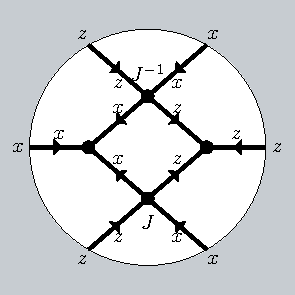
\includegraphics{MagicSquare-figure5.pdf}}
		& \resizebox{0.25\textwidth}{!}{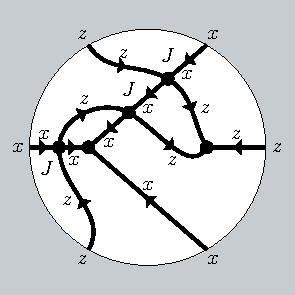
\includegraphics{MagicSquare-figure6.pdf}}
		&$\begin{aligned}[t]
				  &(zx)zxzx\\
				  &=Jxz(zx)zx\\
				  &=J^2x(zx)zzx\\
				  &=xx(zzz)x\\
				  &=(xxx)\\
				  &=1
				\end{aligned}$
		\end{tabular}
	\caption{The first picture uses a minimal number of relations, and corresponds (in an imprecise sense) to the equation manipulations on the left. The second picture corresponds to the equation manipulations on the right, in which each $z$ is commuted all the way to the end of the string.
}
	\label{fig:xz-group-picture}
\end{figure}
\end{example}

\subsection{Representation theory of finite groups}


We'll study groups through their representations. We collect here some basic facts about the representation theory of finite groups. For exposition and proofs, see e.g. \cite{dummit2004abstract}. Throughout, $G$ will be a finite group. It should be noted that some of these facts are not true of infinite groups. 

% \begin{definition}
% 	Let $G$ be a group, $V$ be a $\C$-vector space, and $\m L(V)$ be the group of invertible linear transformations. A \emph{representation} of $G$ is a homomorphism $\rho: G \to \m L(V)$. The \emph{dimension} of $\rho$ is the dimension of $V$ over $\C$. 
% 	% $\rho$ is \emph{self-adjoint} if $\rho(g)^* = \rho(g)$ for all $g$. 
% 	$\rho$ is \emph{unitary} if $\rho(g)^* = \rho(g)\1$ for all $g$. 
% \end{definition}

\begin{definition}
	A $d$-dimensional \emph{representation} of $G$ is a homomorphism from $G$ to the group of invertible linear operators on $\C^d$.
	A representation is \emph{irreducible} if it cannot be decomposed as a direct sum of two representations, each of positive dimension.
	A representation is \emph{trivial} if its image is $\set I$, where $I$ is the identity matrix.
	The \emph{character} of a representation $\s$ is the function defined by $g\mapsto \Tr(\s(g))$. 
	Two representations $\rho_1$ and $\rho_2$ are \emph{equivalent} if there is a unitary $U$ such that for all $g$, $U\rho_1(g) U^\dagger = \rho_2(g)$.
\end{definition}
Notice that a $1$-dimensional representation and its character are the same function, and that $1$-dimensional representations are always irreducible. We sometimes write ``irrep'' for ``irreducible representation.'' The next fact allows us to check equivalence of representations algebraically.

\begin{fact}
	$\rho_1$ is equivalent to $\rho_2$ iff they have the same character. 
\end{fact}
% Implicit in the above fact is that equivalent representations have the same dimension.

The following is immediate:
\begin{lemma}\label{fact:character-convex-combination}
	Let $\s = \bigoplus_i \s_i$ be a direct sum decomposition of $\s$ into irreducibles. Let $\circ$ denote composition of maps, and let $\chi = \Tr\circ \s, \chi_i = \Tr\circ\s_i$ be the characters corresponding to the representations $\s$. Then $\chi = \sum_i \chi_i$. 

	Furthermore, define $\tilde \chi = \frac1{\dim \s}\chi$ and $\tilde\chi_i = \frac1{\dim \s_i} \chi_i$ as the \emph{normalized characters} of $\s,\s_i$. 
	Then the normalized character of $\s$ is a convex combination of the normalized characters of $\s_i$. 
	\begin{equation}
		\tilde \chi = \sum_i \frac{\dim \s_i}{\dim \s}\tilde\chi_i.
	\end{equation}
\end{lemma}

There is a simple criterion to check whether a representation of a finite group is irreducible:
\begin{fact}\label{fact:irreducibility-criterion}
	$\s$ is an irreducible representation of $G$ iff
	\begin{equation}
		\abs G = \sum_{g\in G} \Tr \s(g) \Tr\s(g\1). 
	\end{equation}
\end{fact}

\begin{definition}
	The \emph{commutator subgroup} $[G,G]$ of $G$ is the subgroup generated by all elements of the form $[a,b] := aba\1b\1$ for $a,b\in G$. The \emph{index} $\abs{G:H}$ of a subgroup $H \leq G$ is the number of $H$-cosets in $G$. Equivalently for finite groups, the index is the quotient of the orders $\abs{G:H}= \frac{\abs G}{\abs{H}}$.
\end{definition}

\begin{fact}\label{fact:1-dim-irreps}
	$G$ has a number $\abs{G:[G,G]}$ of inequivalent $1$-dimensional irreducible representations, each of which restricts to the trivial representation on $[G,G]$.
\end{fact}

\begin{fact}\label{fact:character-dimension}
	For a finite group $G$, the size of the group is equal to the sum of the squares of the dimensions of the irreducible representations. In other words, for $R$ any set of inequivalent irreps, 
	\begin{equation}\label{eq:character-dimension}
			\abs G = \sum_{\s \in R} (\dim \s)^2 \text{ iff $R$ is maximal.}
		\end{equation}	
\end{fact}
By ``maximal'', we mean that any irreducible representation is equivalent to one from $R$. This fact can be used to check whether one has a complete classification of the irreducibles of $G$. This is a special case of the following for $x = 1$.
\begin{fact}[Second orthogonality relation for character tables]\label{fact:orthogonality}
	Let $x\in G$. Let $\s$ vary over a maximal set of inequivalent irreps of $G$, and let $n_\s$ be the dimension of $\s$. Then
	\begin{equation}
		\frac 1{\abs G}\sum_\s n_\s\Tr(\s(x)) = \delta_{x,1}.
	\end{equation}
\end{fact}

\begin{fact}[Schur's lemma]\label{fact:schur}
	Let $\tau: G\to U(\C^d)$ be an irrep and $X \in \m L(\C^d)$ be a linear operator. Suppose that $X\tau(g) = \tau(g)X$ for all $g\in G$. Then $X = \lambda I$ is a scalar multiple of identity. 
\end{fact}